\documentclass[tikz,border=8pt]{standalone}
\usepackage{amsmath,amssymb}
\usepackage{tikz}
\usetikzlibrary{positioning,arrows.meta,calc}

\begin{document}
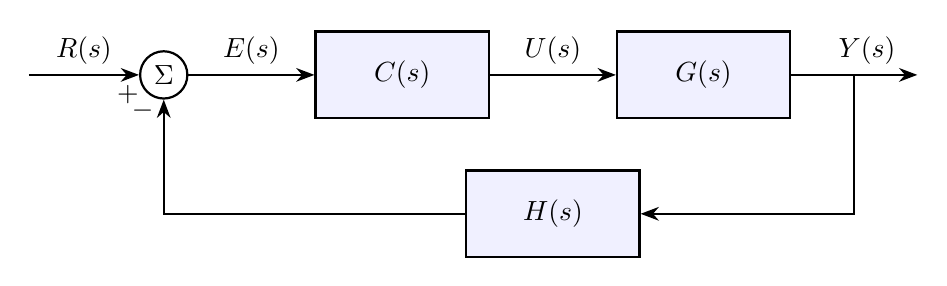
\begin{tikzpicture}[
  node distance=1.6cm, >={Stealth},
  block/.style={draw, thick, rectangle, minimum height=1.1cm, minimum width=2.2cm, fill=blue!6},
  sum/.style={draw, thick, circle, inner sep=0pt, minimum size=6mm},
]
  \coordinate (in);
  \node[sum, right=1.4cm of in] (s) {$\Sigma$};
  \node[block, right=of s] (c) {$C(s)$};
  \node[block, right=of c] (g) {$G(s)$};
  \coordinate[right=1.6cm of g] (out);
  \node[block, below=1.2cm of $(c)!0.5!(g)$] (h) {$H(s)$};

  \draw[->, thick] (in) -- node[above] {$R(s)$} node[pos=0.9, below] {$+$} (s);
  \draw[->, thick] (s) -- node[above] {$E(s)$} (c);
  \draw[->, thick] (c) -- node[above] {$U(s)$} (g);
  \draw[->, thick] (g) -- node[above, pos=0.6] {$Y(s)$} (out);
  \draw[->, thick] ($(g.east)!0.5!(out)$) |- (h);
  \draw[->, thick] (h) -| node[pos=0.95, left] {$-$} (s);
\end{tikzpicture}
\end{document}
